\documentclass[Lecture.tex]{subfiles}
\begin{document}
\section{5.3: Area Between Two Curves}

\begin{frame}{Motivation}
  Say we wanted to find the area between the two curves
  $$f(x) = x^2\ \text{and}\ g(x) = x$$
  on the interval $[0,1]$.
  \onslide<2->{Geometrically, this is obvious: compute the bigger area, then subtract the smaller area.}
\end{frame}

\begin{frame}{Motivation (Cont.)}
  The area under the line:
  \begin{center}
    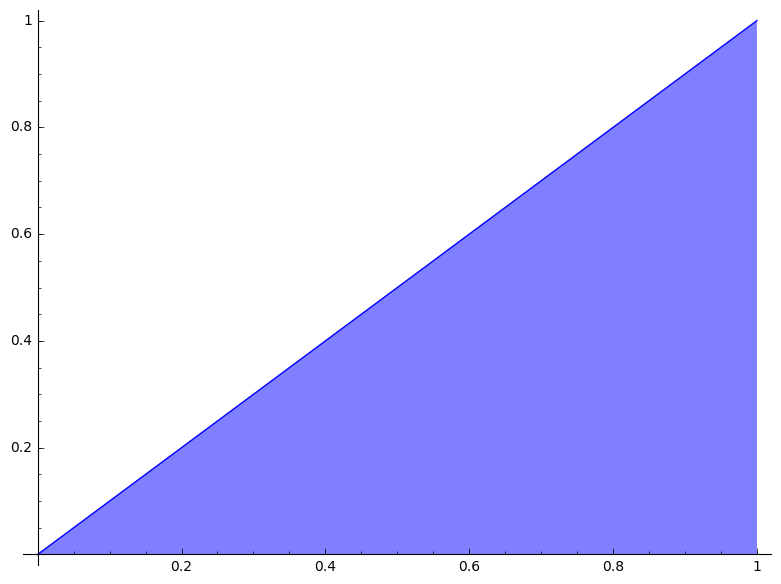
\includegraphics[scale=0.3]{topArea}
  \end{center}
\end{frame}
\begin{frame}
  The area under the parabola:
  \begin{center}
    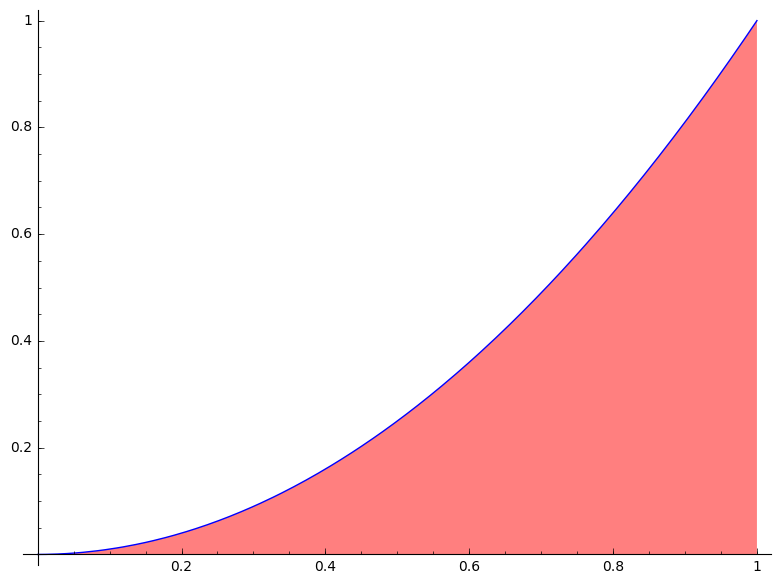
\includegraphics[scale=0.3]{bottomArea}
  \end{center}
\end{frame}

\begin{frame}{Motivation (Cont.)}
  On one plot:
  \begin{center}
    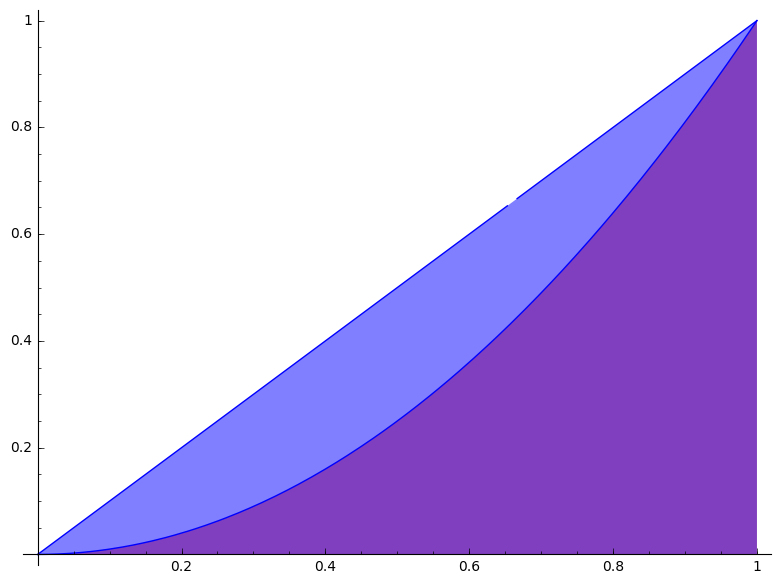
\includegraphics[scale=0.25]{areaBetweenLineAndParabola}
  \end{center}
  The blue area is what we want to compute.
  The purple area is the intersection of the red solid and the blue solid; this is the area we want to remove from the area under the line.
\end{frame}

\begin{frame}{Motivation (Cont.)}
  So, all we need to do is compute
  \begin{eqnarray*}
    \onslide<2->{\int_0^1 x \dx{x} - \int_0^1 x^2 \dx{x}}
    \onslide<3->{&=& \frac{1}{2}x^2\Big|_0^1 - \frac{1}{3}x^3\Big|_0^1\\}
    \onslide<4->{&=& \frac{1}{2}(1 - 0) - \frac{1}{3}(1 - 0)\\}
    \onslide<5->{&=& \frac{3}{6} - \frac{2}{6}\\}
    \onslide<6->{&=& \frac{1}{6}.}
  \end{eqnarray*}
\end{frame}

\begin{frame}{Area Between Two Curves}
  Assume that $f$ and $g$ are continuous functions on $[a,b]$ and that $g(x) \leq f(x)$ for all $a \leq x \leq b$.
  The area between the two curves is
  $$\int_a^b f(x) - g(x)\dx{x} = \int_a^b f(x)\dx{x} - \int_a^bg(x)\dx{x}.$$
\end{frame}

\begin{frame}{Example}
  Find the area between $f(x) = 4x - x^2$ and $g(x) = \frac{1}{2}x^{\frac{3}{2}}$ for $0 \leq x$.
  \onslide<2->{
    First we must figure out where these intersect.
  }
  \onslide<3->{
    So, we must solve
    $$4x - x^2 = \frac{1}{2}x^{\frac{3}{2}}$$
    for $x$:
    }
  \begin{eqnarray*}
    \onslide<4->{4x - x^2 &=& \frac{1}{2}x^{\frac{3}{2}}\\}
    \onslide<5->{\Rightarrow x(4 - x) &=& x\left(\frac{\sqrt{x}}{2}\right)}
  \end{eqnarray*}
  \onslide<6->{
    implies either $x = 0$ or $4 - x = \frac{1}{2}\sqrt{x}$.
  }
  \onslide<7->{
    The latter is equivalent to solving 
  $$2x + \sqrt{x} - 8 = 2\sqrt{x}^2 + \sqrt{x} - 8 = 0.$$
  }
\end{frame}

\begin{frame}{Example (Cont.)}
  We can solve $2\sqrt{x}^2 + \sqrt{x} - 8 = 0$ using the Quadratic Formula:
  \begin{eqnarray*}
    \onslide<2->{\sqrt{x} &=& \frac{-1 \pm \sqrt{1 - (4)(2)(-8)}}{2(2)}\\}
    \onslide<3->{&=& \frac{-1 \pm \sqrt{1 + 64}}{4}\\}
    \onslide<4->{&=& \frac{-1 \pm \sqrt{65}}{4}.}
  \end{eqnarray*}
  \onslide<5->{
    Since $\sqrt{x}$ is positive, the only solution is
    $$\sqrt{x} = \frac{-1 + \sqrt{65}}{4}.$$
    }
  \onslide<6->{
    Hence
    $$x = \left(\frac{-1 + \sqrt{65}}{4}\right)^2 \approx 3.11$$
  }
\end{frame}

\begin{frame}{Example (Cont.)}
  The plot of the two functions is
  \begin{center}
    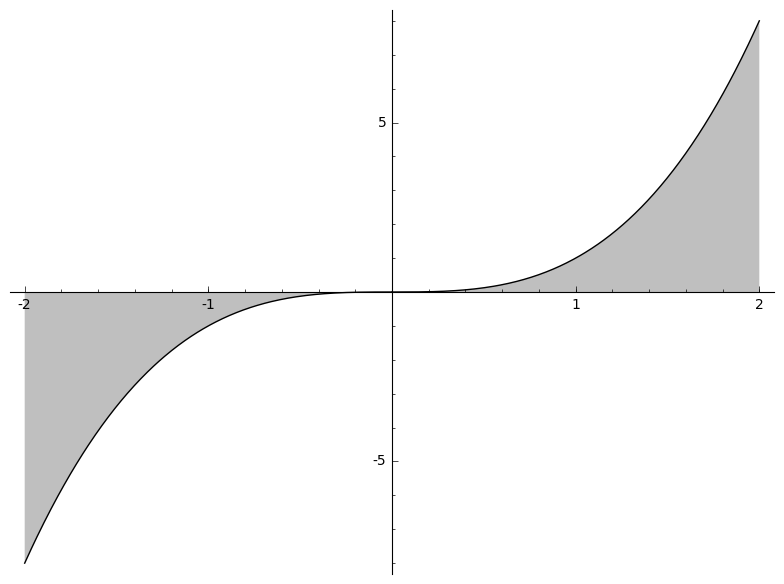
\includegraphics[scale=0.3]{areaBetweenCurves}
  \end{center}
  The parabola, $f(x)$ is on top, and $g(x)$ is the bottom curve.
\end{frame}

\begin{frame}{Example (Cont.)}
  If we let 
  $$b = \left(\frac{-1 + \sqrt{65}}{4}\right)^2$$
  then the area between these two curves is given by
  \scalebox{.75}{\parbox{\linewidth}{
  \begin{eqnarray*}
    \onslide<2->{\int_0^b f(x) - g(x)\dx{x} &=&}
    \onslide<3->{\int_0^b 4x - x^2 - \frac{1}{2}x^{\frac{3}{2}}\dx{x}\\}
    \onslide<4->{&=& 4\int_0^b x \dx{x} - \int_0^b x^2 \dx{x} - \frac{1}{2}\int_0^b x^{\frac{3}{2}}\dx{x}\\}
    \onslide<5->{&=& 2x^2\Big|_0^b - \frac{1}{3}x^3\Big|_0^b - \frac{1}{5}x^{\frac{5}{2}}\Big|_0^b}\\
    \onslide<6->{&=& 2\left(\frac{-1 + \sqrt{65}}{4}\right)^4 - \frac{1}{3}\left(\frac{-1 + \sqrt{65}}{4}\right)^6 - \frac{1}{5}\left(\frac{-1 + \sqrt{65}}{4}\right)^5\\}
    \onslide<7->{&\approx& 5.91.}
  \end{eqnarray*}
  }}
\end{frame}
\end{document}
